\documentclass{report}
\usepackage{graphicx}
\graphicspath{ {} }
\usepackage[portuges]{babel}
\usepackage{hyperref}
\usepackage{listings}
\usepackage{url}
\usepackage{soul}
\usepackage{subcaption}
\parindent=0pt
\parskip=2pt

\usepackage{listings}
\usepackage{color}

\definecolor{dkgreen}{rgb}{0,0.6,0}
\definecolor{gray}{rgb}{0.5,0.5,0.5}
\definecolor{mauve}{rgb}{0.58,0,0.82}

\lstset{frame=tb,
  language=C++,
  aboveskip=3mm,
  belowskip=3mm,
  showstringspaces=false,
  columns=flexible,
  basicstyle={\scriptsize\ttfamily},
  numbers=none,
  numberstyle=\tiny\color{gray},
  keywordstyle=\color{blue},
  commentstyle=\color{dkgreen},
  stringstyle=\color{mauve},
  breaklines=true,
  breakatwhitespace=true,
  tabsize=2
}


\title{Computa\c{c}\~ao Gr\'afica \\ \setlength{\baselineskip}{1.5\baselineskip} \textbf{Primitivas Gr\'aficas} \\ Relat\'orio de Desenvolvimento}
\author{ Jo\~ao Manuel Martins Cerqueira (A65432) \and S\'onia Catarina Guerra Costa (A71506) \and Tiago Costa Loureiro (A71191)}
\date{Ano letivo 2016/2017}

\begin{figure}
\centering
\includegraphics[scale=0.3]{logo_eeng.png}
\end{figure}

\begin{document}

\maketitle 

\tableofcontents

% CAPITULO 1

\chapter{Introdu\c{c}\~{a}o}
 
Este trabalho pr\'atico est\'a dividido em duas partes. Uma primeira parte onde \'e pedido que se desenvolva um gerador de v\'ertices de tri\^angulos necess\'arios para criar as formas geom\'etricas primitivas e guard\'a-los num ficheiro .3d. E uma segunda etapa onde o principal objetivo \'e o desenvolvimento de um motor capaz de ler um ficheiro XML com o nome dos ficheiros .3d onde os v\'ertices do modelo a desenvolver est\~ao guardados e assim criar as formas geom\'etricas primitivas pretendidas.

\section{Estrutura do documento}
A estrutura que este relat\'orio segue, excluindo o presente cap\'itulo onde se faz uma pequena introdu\c{c}\~{a}o do assunto, é: 
\begin{itemize}
\item No cap\'itulo 2 faz-se uma an\'alise detalhada do problema proposto de modo a poder-se especificar as entradas, resultados e formas de transforma\c{c}\~{a}o.
\item No cap\'itulo 3 faz-se referencia \`a conce\c{c}\~{a}o/desenho da Resolu\c{c}\~{a}o dos problemas propostos, mostrando assim as estruturas de dados e todos os algoritmos usados durante a realiza\c{c}\~{a}o deste trabalho.
\item No cap\'itulo 4 faz-se refer\^encia a decis\~{o}es e problemas de implementa\c{c}\~{a}o que surgiram. 
\item No cap\'itulo 5 faz-se uma conclus\~{a}o / s\'intese de todo o trabalho realizado e uma an\'alise cr\'itica dos resultados.
\item Em ap\^endice faz-se uma refer\^encia ao c\'odigo necess\'ario para a implementa\c{c}\~{a}o do programa.
\end{itemize}
Este trabalho \'e finalizado com a Bibliografia que cont\^em todas as refer\^encias biliogr\'aficas usadas na realiza\c{c}\~{a}o do mesmo.

%\section{Ambiente de Trabalho utilizado}
% CAPITULO 2
\chapter{An\'alise e Especifica\c{c}\~{a}o} 
\section{Especifica\c{c}\~{a}o do Problema} % 2.1
Primeiramente será desenvolvido um Gerador em C++ que recebe como argumentos os dados necess\'arios para a cria\c{a}\~ao de uma figura. Após processar os dados, o programa imprime num ficheiro .3d, cujo nome \'e dado como argumento, todos os v\'ertices dos tri\^angulos precisos para gerar uma figura. Este gerador é capaz de desenvolver os vértices dos tri\^angulos para as seguintes figuras:
\begin{itemize}
\item Plano, sendo este um quadrado no plano XZ, centrado na origem, feito com dois tri\^angulos;
\item Caixa, definido pelas dimens\~oes de X, Y e Z e opcionalmente pelo n\'umero de divis\~oes;
\item Esfera, definida por raio, fatias e camadas;
\item Cone, definido pelo raio da base, pela altura, fatias e camadas.
\end{itemize}

A segunda parte do trabalho consiste no desenvolvimento de um Motor em C++. Este motor recebe como argumento um ficheiro XML. Neste ficheiro XML est\~ao guardados nomes de ficheiros .3d onde anteriormente foram guardados v\'ertices de uma figura. Ao abrir e processar esses mesmos ficheiros ser\'a criada uma cena em 3 dimens\~oes a partir desses mesmos v\'ertices. Neste m\'odulo encontram-se as informa\c{c}\~oes sobre a c\^amara utilizada e tamb\'em est\~ao definidas as fun\c{c}\~ao que permitem a intera\c{c}\~ao do utilizador com o cen\'ario final.
\begin{figure}[h]
\centering
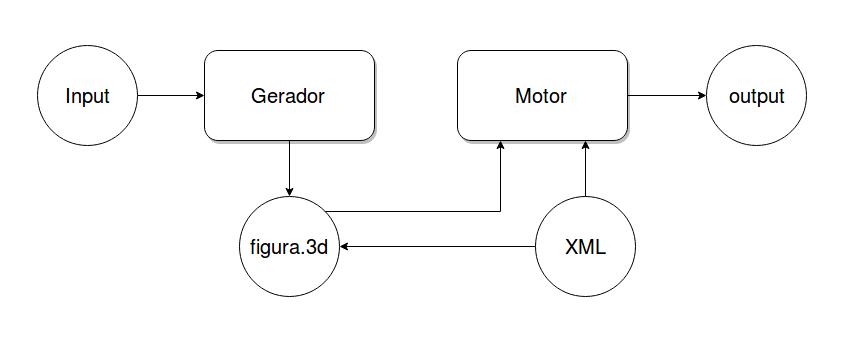
\includegraphics[scale=0.4]{diagrama.png}
\caption{Diagrama do trabalho}
\end{figure}
% CAPITULO 3
\chapter{Conce\c{c}\~{a}o/Desenho da Resolu\c{c}\~{a}o} 
\section{Desenvolvimento do Gerador} % 3.1 - 
Este m\'odulo tem como input os par\^ametros necess\'arios para a cria\c{c}\~ao dos modelos pretendidos (como se pode ver no exemplo abaixo) e tamb\'em recebe como \'ultimo par\^ametro o nome do ficheiro criado como output. Se n\~ao for dado nenhum par\^ametro ou at\'e mesmo dados par\^ametros errados, o programa sai com mensagem de erro. 
\begin{lstlisting}
   $ gerador plane 4 plano.3d
\end{lstlisting}

Inicialmente imprime-se no ficheiro .3d o n\'umero de tri\^angulos cujos v\'ertices ser\~ao impressos.
Para desenvolver o Gerador \'e preciso perceber como s\~ao criadas as figuras a partir de tri\^angulos.
\begin{figure}[h]
\centering
\includegraphics[scale=0.6]{exemplo_output_plano.png}
\caption{Exemplo de output de plano.3d}
\end{figure}
\\
\\
\subsection{Plano}
Para construir o plano, a fun\c{c}\~ao recebe um \'unico par\^ametro, a sua dimens\~ao.
Como \'e referido no enunciado, sabe-se que o plano \'e quadrado e que se encontra
no plano XZ, restringindo as coordenadas de y a zero sendo apenas necess\'ario calcular as coordenadas x e z. Sendo o 
plano quadrado e centrado na origem, rapidamente se chega que a
coordenada x tem os valores x/2 ou -x/2 e a coordenada z \'eé an\'aloga.
Ou seja, os 4 pontos do plano s\~ao (-x/2, 0, -z/2), (-x/2, 0, z/2),
(x/2, 0, -z/2) e (x/2,0,z/2).
\begin{figure}[h]
\centering
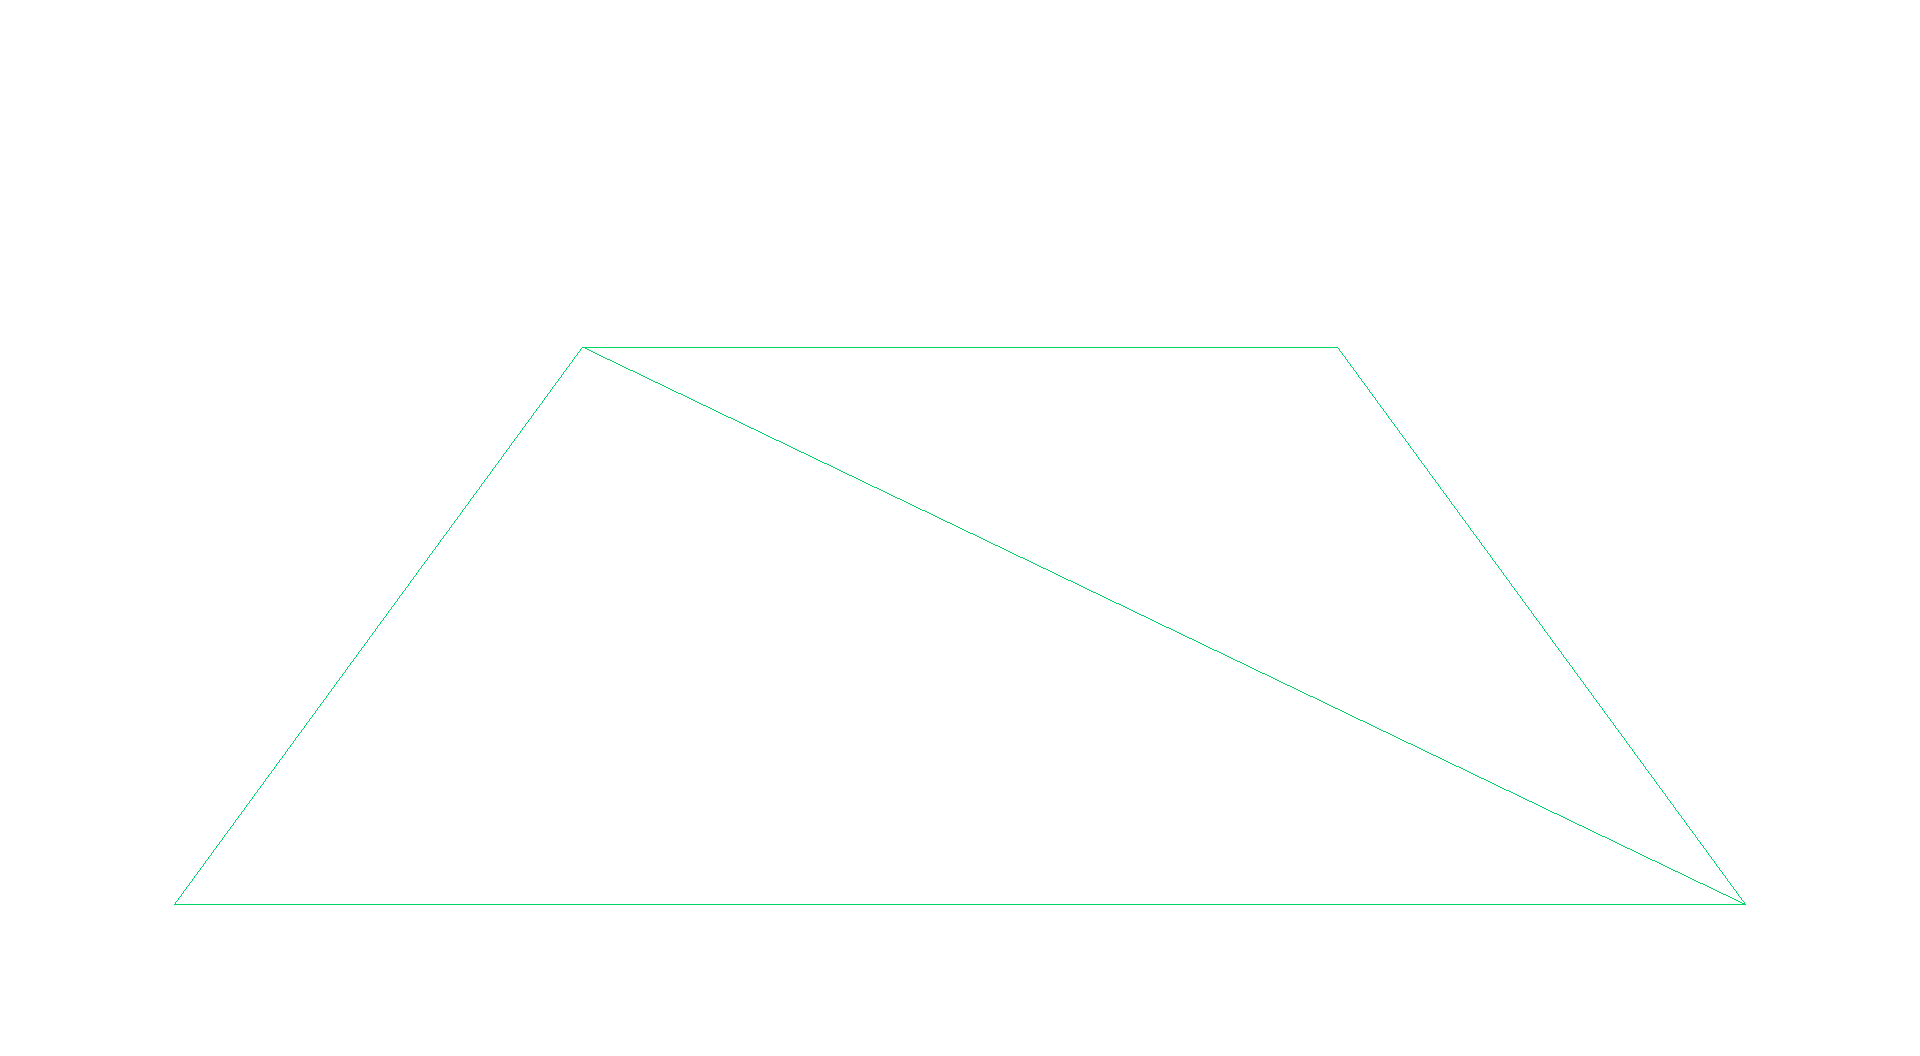
\includegraphics[scale=0.15]{plano.png}
\caption{Exemplo plano}
\end{figure}
\clearpage
\subsection{Caixa}
No desenho da caixa come\c{c}a-se por receber as suas dimens\~oes x, y e z e ainda o n\'umero de dimens\~oes. Pretende-se desenhar a caixa centrada no ponto que o motor escolheu, por isso come\c{c}a por calcular o seu ponto de origem. Sabendo as dimens\~oes da caixa, facilmente percebemos que o seu ponto de origem é o ponto (-x/2, -y/2, -z/2). Sabemos tamb\'em que na diagonal oposta temos o ponto (x/2, y/2, z/2). De seguida, calcula-se qual as dimens\~oes x, y e z que cada tri\^angulo ter\'a e estas s\~ao guardadas nas vari\'aveis dim\_x, dim\_y e dim\_z respectivamente.
Seguidamente, cria-se a caixa a partir do ponto de origem, desenhando as tr\^es faces conectadas a esse ponto. Come\c{c}ando em (-x/2, -y/2, -z/2) desenhamos os tri\^angulos conectados a esse ponto e em seguida avan\c{c}-se para o pr\'oximo ponto em z. Depois de percorrermos todos os pontos de (-x/2, -y/2, -z/2) até (-x/2, -y/2, z/2) subimos para a próxima coordenada em y e recome\c{c}a-se a coordenada z em –z/2, at\'e ao ponto (-x/2, y/2, z/2). Ap\'os este passo, todos os pontos para x = -x/2 foram percorridos e, de forma an\'aloga aos passos anteriores passamos para a pr\'oxima coordenada de x at\'e que eventualmente tenham sido desenhadas todas as 3 faces conectadas ao ponto de origem. Ap\'os serem desenhadas estas 3 faces, faz-se de forma an\'aloga para as outras 3 faces partindo agora do ponto (x/2, y/2, z/2) e em vez de incrementar para andar nos eixos x, y e z decrementa-se de acordo com as dimens\~oes de cada tri\^angulo.

\begin{figure}[h]
\centering
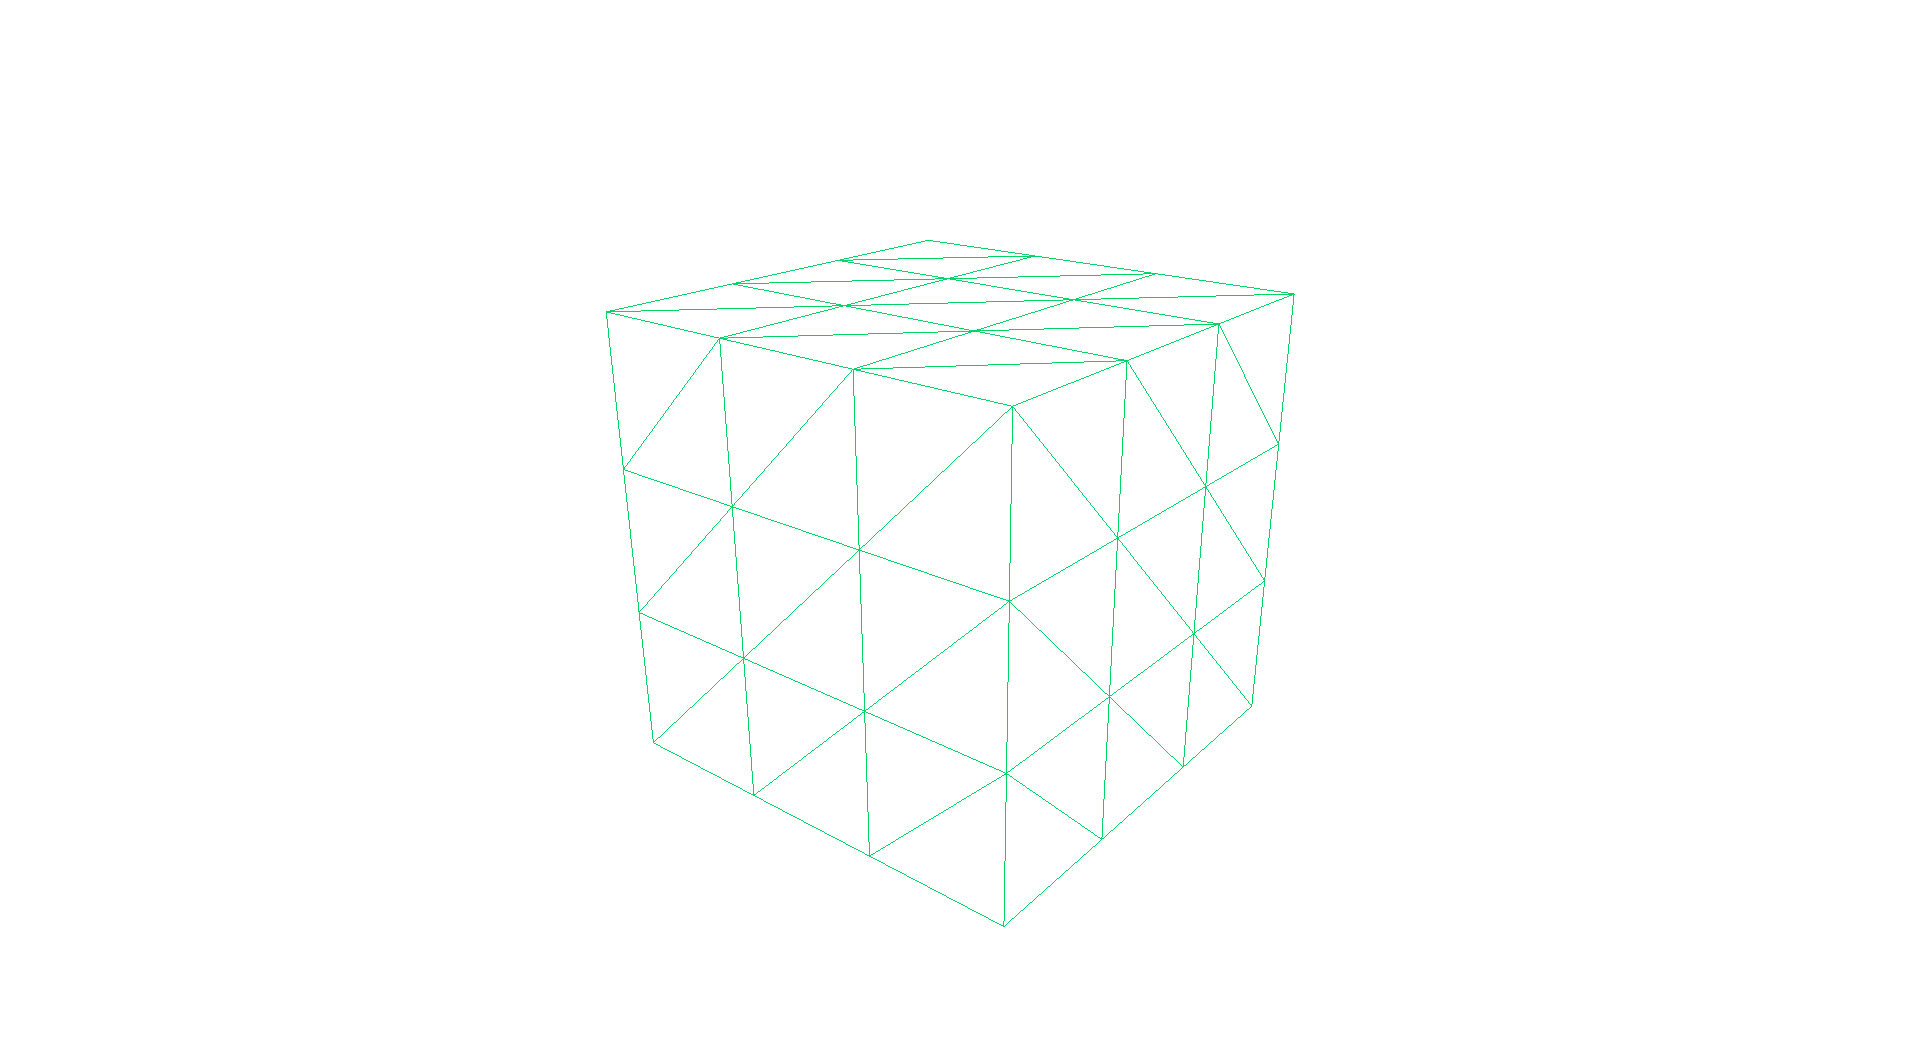
\includegraphics[scale=0.15]{caixa.png}
\caption{Exemplo Caixa}
\end{figure}
\clearpage
\subsection{Esfera}
Para desenhar a esfera recebe-se como par\^ametros o raio da esfera e o n\'umero de fatias e camadas. Inicialmente calcula-se o \^angulo de cada fatia e camada. De seguida, come\c{c}a-se a  desenhar a esfera a partir do centro e em dire\c{c}\~ao ao topo e \'a base. Primeiro calcula-se os raios de cada fatia e camada, juntamente com os \^angulos de cada uma em rela\c{c}\~ao \'as primeiras. Com os raios e com os \^angulos obtem-se os 3 pontos de cada tri\^angulo.

\begin{figure}[h]
\centering
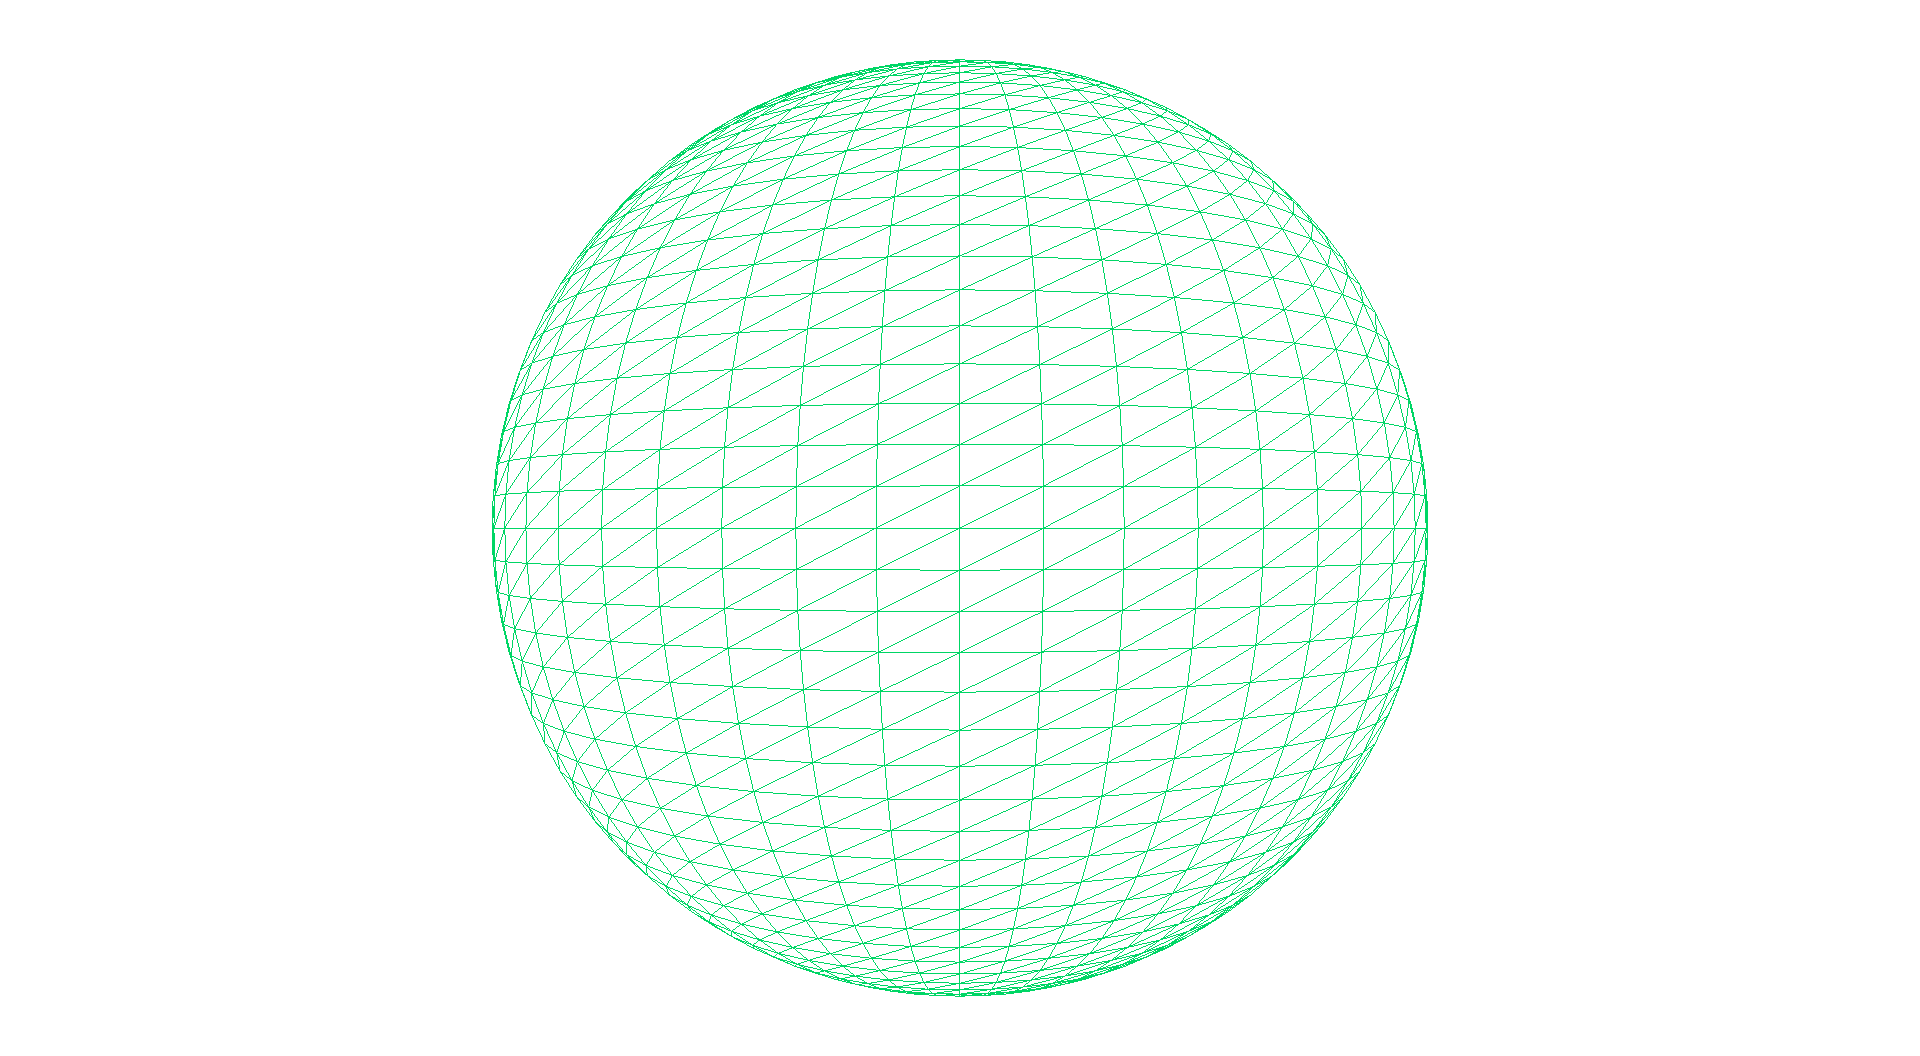
\includegraphics[scale=0.15]{esfera.png}
\caption{Exemplo Esfera}
\end{figure}
\clearpage
\subsection{Cone}
Para a constru\c{c}\~ao do cone s\~ao dados como par\^ametros o raio da base, a altura do cone e n\'umero de camadas e fatias. Primeiro \'e calculado \^angulo de cada fatia e de cada camada e ainda a altura de cada camada. De seguida calcula-se o raio da pr\'oxima camada e, usando esse raio, o raio da primeira base e os ângulos de cada camada e fatia, obtem-se a coordenada x e z de cada ponto e com a altura da camada obtem-se o ponto y.

\begin{figure}[h]
\centering
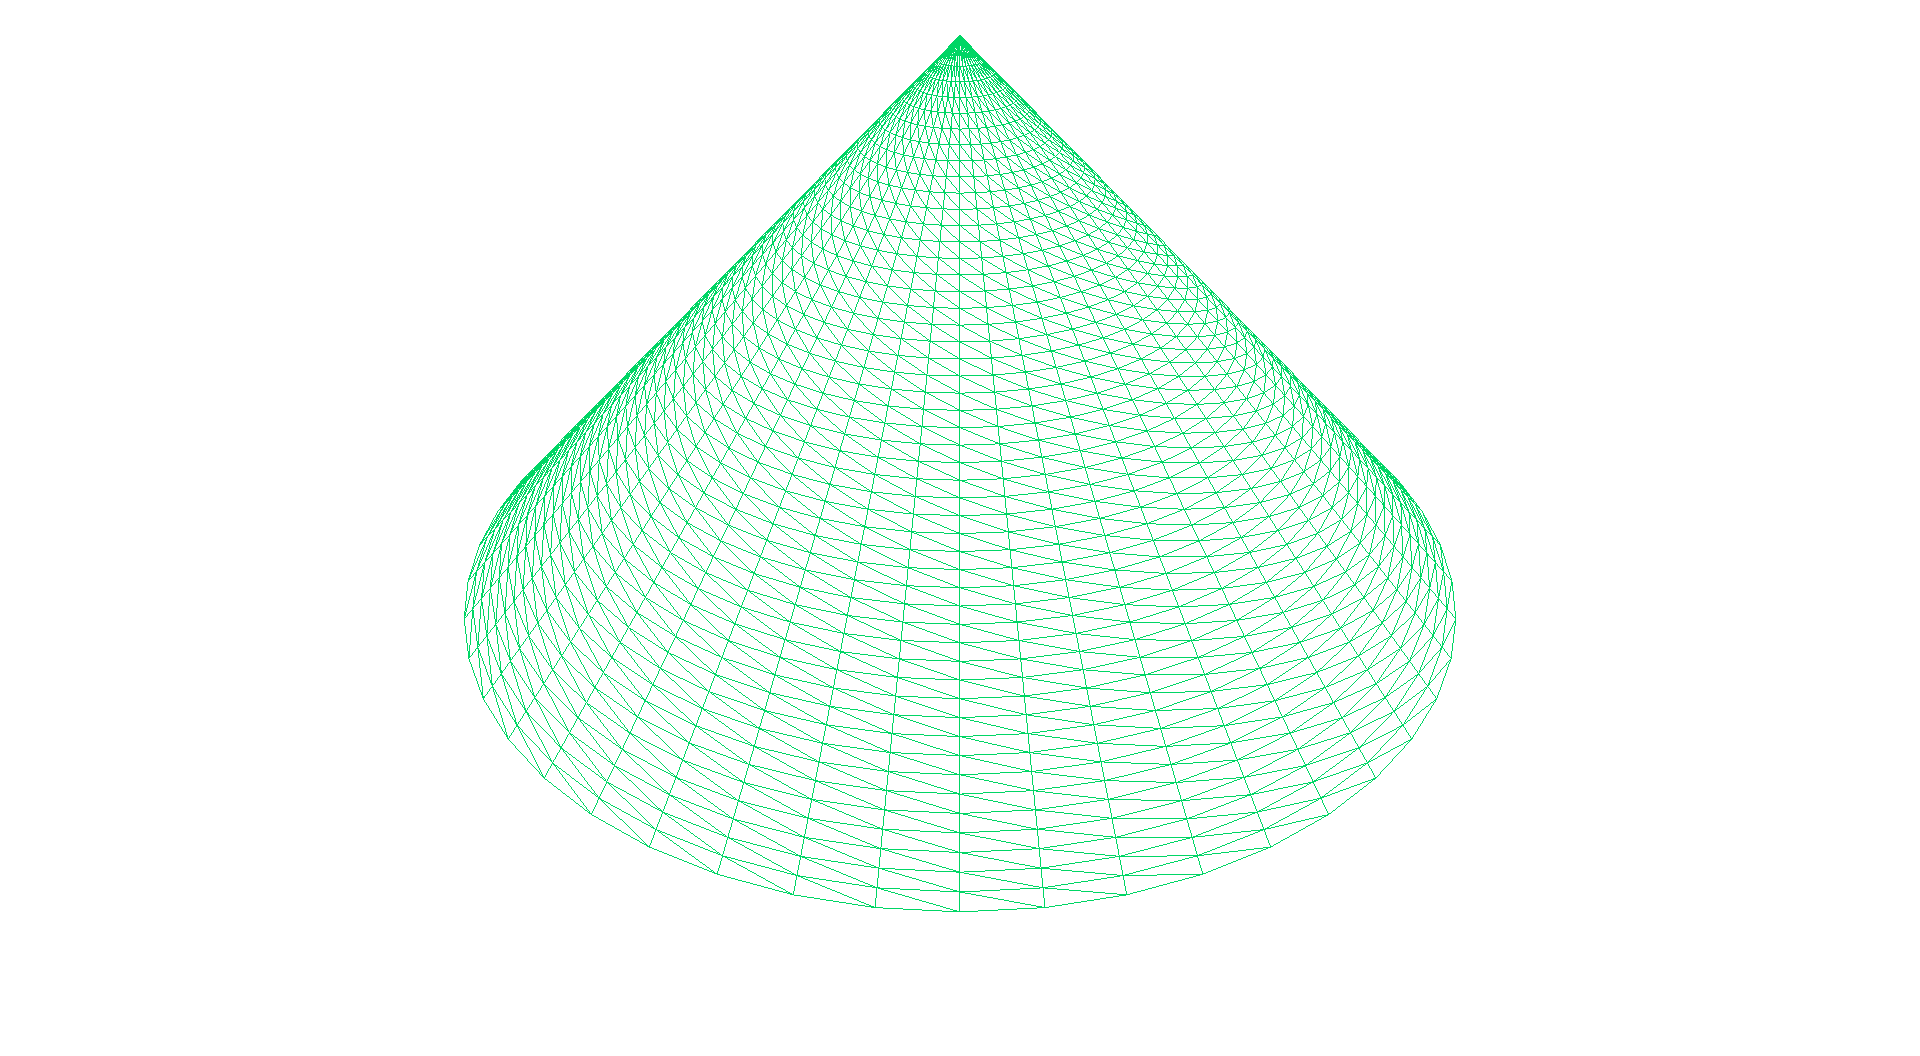
\includegraphics[scale=0.15]{cone.png}
\caption{Exemplo Cone}
\end{figure}
\\
\clearpage
\section{Desenvolvimento do Motor}
O motor apresenta um dos principais problemas desta primeira fase devido \`a necessidade de aprender a manipular os ficheiros XML.
A estrat\'egia optada foi primeiro receber o ficheiro XML como argumento e de seguida, com a função le\_xml(char *nome) que recebe o nome do ficheiro obtendo todos os nomes dos ficheiros .3d que constituem a cena e s\~ao guardados num vector chamado lista\_ficheiros.    
Ap\'os isso, na função renderScene() \'e chamada a fun\c{c}\~ao desenha(). Esta \'ultima vai ler os nomes dos ficheiros .3d que est\~ao no vector lista\_ficheiros e a partir desses nomes abre os ficheiros correspondentes e desenha os tri\^angulos representados pelos v\'ertices que est\~ao nos ficheiros, atribuindo cores aleat\'orias a cada figura. \newline

\begin{figure}[h]
\centering
\includegraphics[scale=0.15]{cena.png}
\caption{Output do Motor}
\end{figure}

% CAPITULO 4
\chapter{Codifica\c{c}\~{a}o e Testes} % 4.1
\section{Problemas de Implementa\c{c}\~{a}o}
No desenho das figuras surgiram alguns problemas. 
Na constru\c{c}\~ao da caixa apenas foi poss\'ivel desenhar a figura recorrendo a 6 ciclos (for) e 6 condi\c{c}\~oes (if), os quais percorrem todos os pontos poss\'iveis da caixa, incluindo os interiores. Uma vez que n\~ao se quer desenhar dentro da caixa (apenas desenhar a superf\'icie) n\~ao ser\'ia necess\'ario percorrer todos os pontos. Contudo foi a \'unica solu\c{c}\~ao encontrada dados os requisitos.
O cone tamb\'em suscitou algumas d\'uvidas, pelo facto de ser necess\'ario calcular o raio a cada camada. Numa primeira tentativa, calculou-se o raio de acordo com o raio da base e o cosseno do \^angulo da stack, contudo a figura ficava com superf\'icies curvas. 
\clearpage
\section{Compila\c{c}\~ao}
Para que o progrma seja de f\'acil acesso a qualquer utilizador, foi criada uma makefile que permite executar todo o programa desde o input at\'e \`a constru\c{c}\~ao final das figuras em 3 dimens\~oes. Foi criado tamb\'em um ficheiro readme.md que explica da seguinte forma como executar.
\subsection{Como executar}
No terminal escrever make e a makefile vai gerar os ficheiros .3d com as seguintes propriedades:
%%%%%%%%%%%%%%%%%%%%%%%%%%%%%%%%%%%%%%%%%%%%%%%%%%%%%%%%%%%%%%%%%%%%%%%%%%%%%%%%%%%%%%%%%%%%%%%%%%%%%
\begin{itemize}
    \item plane
        \begin{itemize}
            \item comprimento = 4
            \item nome do ficheiro = plane.3d
        \end{itemize}
    \item box
        \begin{itemize}
            \item tamanho X = 2
            \item tamanho Y = 2
            \item tamanho Z = 2
            \item n\'umero de divis\~oes = 3
            \item nome do ficheiro = box.3d
        \end{itemize}
    \item sphere
        \begin{itemize}
            \item raio = 2
            \item fatias  = 50
            \item camadas = 50
            \item nome do ficheiro = sphere.3d
        \end{itemize}
    \item cone
        \begin{itemize}
            \item raio da base = 2
            \item altura = 2
            \item fatias = 50
            \item camadas = 50
            \item nome do ficheiro = cone.3d
        \end{itemize}
\end{itemize}
\clearpage
De seguida \'e executado o motor com o argumento "configuracao.xml", que cont\'em esta informa\c{c}\~ao:
\begin{lstlisting}
<scene>
  <model file="plane.3d" />
  <model file="cone.3d" />
  <model file="sphere.3d" />
  <model file="box.3d" />
</scene>
\end{lstlisting}
\subsection{Gerador}
Os ficheiros .3d são gerados na pasta principal do motor.
\begin{itemize}
\item Argumentos:
\begin{itemize}
    \item Plane
        \begin{itemize}
            \item Comprimento
            \item Nome do ficheiro para guardar
        \end{itemize}
    \item Box
        \begin{itemize}
            \item Tamanho X
            \item Tamanho Y
            \item Tamanho Z
            \item N\'umero de divis\~oes(opcional|default = 1)
            \item Nome do ficheiro para guardar
        \end{itemize}
    \item Sphere
        \begin{itemize}
            \item Raio
            \item Fatias
            \item Camadas
            \item Nome do ficheiro para guardar
        \end{itemize}
    \item Cone
        \begin{itemize}
            \item Raio da base
            \item Altura
            \item Fatias
            \item Camadas
            \item Nome do ficheiro para guardar
        \end{itemize}
\end{itemize}

\end{itemize}
\clearpage
\subsection{Motor}
\begin{itemize}
\item Argumentos:
    \begin{itemize}
        \item Nome do ficheiro .xml (procura dentro da pasta xml que está na pasta motor)
    \end{itemize}
\item Op\c{c}\~oes do menu:
    \begin{itemize}
        \item Fill 
            \begin{itemize}
                \item glPolygonMode(GL\_FRONT\_AND\_BACK,GL\_FILL);
            \end{itemize}
        \item Line
            \begin{itemize}
                \item glPolygonMode(GL\_FRONT\_AND\_BACK,GL\_LINE);
            \end{itemize}
        \item Point
            \begin{itemize}
                \item glPolygonMode(GL\_FRONT\_AND\_BACK,GL\_POINT);
            \end{itemize}
        
    \end{itemize}
\item Teclado
    \begin{itemize}
        \item Seta cima
            \begin{itemize}
                \item roda para cima
            \end{itemize}
        \item Seta baixo
            \begin{itemize}
                \item roda para baixo
            \end{itemize}
        \item Seta direita
            \begin{itemize}
                \item roda para a direita
            \end{itemize}
        \item Seta esquerda
            \begin{itemize}
                \item roda para a esquerda
            \end{itemize}
        \item Page up
            \begin{itemize}
                \item aproxima os objetos
            \end{itemize}
        \item Page down
            \begin{itemize}
                \item afasta os objetos
            \end{itemize}
    \end{itemize}
\end{itemize}
% CAPITULO 5

\chapter{Conclus\~{a}o}
O presente relat\'orio teve como objetivo explicar todo o processo de constru\c{c}\~ao de um cen\'ario em 3 dimens\~oes desde o input do utilizador at\'e ao output.
Neste trabalho, que envolve a constru\c{c}\~ao de modelos gr\'aficos primitivos atrav\'es de tri\^angulos, n\~ao foram usados os m\'etodos mais eficientes, o que n\~ao aconteceria se fossem usados VBO's, algo que ser\'a implementado numa pr\'oxima fase. 
\newline
%%%%%%%%%%%%%%%%%%%%%%%%%%%%%%%%%%%%%%%%%%%%%%%%%%%%%%%%%%%%%%%%%%%%%%%%%%%%%%%%%%%%%%%%%%%%%%%%%%%%%%%
\appendix
\chapter{C\'odigo do Programa}
\section{C\'odigo Gerador}
\begin{lstlisting}
#include <iostream>
#include <fstream>
#include <math.h>

using namespace std;

fstream file;

void plano(float comprimento){
    float m_comp = comprimento/2;

    // Nº DE TRIANGULOS
    file << "2" << endl;

    file << -m_comp << " 0.0 " << -m_comp << endl;
    file << -m_comp << " 0.0 " << m_comp << endl;
    file << m_comp << " 0.0 " << m_comp << endl;

    file << m_comp << " 0.0 " << m_comp << endl;
    file << m_comp << " 0.0 " << -m_comp << endl;
    file << -m_comp << " 0.0 " << -m_comp << endl;

}

void caixa(float x, float y, float z,  int dimensions){
    double dim_x = x / dimensions, dim_y = y / dimensions, dim_z = z / dimensions;
    double ori_x = -x / 2, ori_y = -y / 2, ori_z = -z / 2; // origem x, y e z
    double xx = ori_x, yy = ori_y, zz = ori_z; // ponto "origem"

    file << 4 << endl;

    for (xx = ori_x; xx < (-ori_x); xx += dim_x) {
        //x2 = x1 + dim_x;

        for (yy = ori_y; yy < (-ori_y); yy += dim_y) {
            //y2 = y1 + dim_y;

            for (zz = ori_z; zz < (-ori_z); zz += dim_z) {
                //z2 = z1 + dim_z;

                if (xx == ori_x) {
                    //glColor3f(0.09 << " " << 0.5 << " " << 0.99 << endl;
                    file << xx << " " << yy + dim_y << " " << zz << endl;
                    file << xx << " " << yy << " " << zz << endl;
                    file << xx << " " << yy + dim_y << " " << zz + dim_z << endl;

                    //glColor3f(0.18 << " " << 0.5 << " " << 0.90 << endl;
                    file << xx << " " << yy + dim_y << " " << zz + dim_z << endl;
                    file << xx << " " << yy << " " << zz << endl;
                    file << xx << " " << yy << " " << zz + dim_z << endl;

                }

                if (yy == ori_y) {
                    //glColor3f(0.27 << " " << 0.5 << " " << 0.81 << endl;
                    file << xx << " " << yy << " " << zz << endl;
                    file << xx + dim_x << " " << yy << " " << zz << endl;
                    file << xx + dim_x << " " << yy << " " << zz + dim_z << endl;

                    //glColor3f(0.36 << " " << 0.5 << " " << 0.73 << endl;
                    file << xx + dim_x << " " << yy << " " << zz + dim_z << endl;
                    file << xx << " " << yy << " " << zz + dim_z << endl;
                    file << xx << " " << yy << " " << zz << endl;
                }

                if (zz == ori_z) {
                    //glColor3f(0.45 << " " << 0.5 << " " << 0.64 << endl;
                    file << xx << " " << yy << " " << zz << endl;
                    file << xx << " " << yy + dim_y << " " << zz << endl;
                    file << xx + dim_x << " " << yy << " " << zz << endl;

                    //glColor3f(0.54 << " " << 0.5 << " " << 0.55 << endl;
                    file << xx + dim_x << " " << yy << " " << zz << endl;
                    file << xx << " " << yy + dim_y << " " << zz << endl;
                    file << xx + dim_x << " " << yy + dim_y << " " << zz << endl;
                }
            }
        }
    }

    for (xx = -ori_x; xx > ori_x; xx -= dim_x) {
        for (yy = -ori_y; yy > ori_y; yy -= dim_y) {
            for (zz = -ori_z; zz > ori_z; zz -= dim_z) {
                if (xx == -ori_x) {
                    //glColor3f(0.63 << " " << 0.63 << " " << 0.46 << endl;
                    file << xx << " " << yy << " " << zz << endl;
                    file << xx << " " << yy - dim_y << " " << zz << endl;
                    file << xx << " " << yy - dim_y << " " << zz - dim_z << endl;

                    //glColor3f(0.72 << " " << 0.72 << " " << 0.37 << endl;
                    file << xx << " " << yy - dim_y << " " << zz - dim_z << endl;
                    file << xx << " " << yy << " " << zz - dim_z << endl;
                    file << xx << " " << yy << " " << zz << endl;

                }

                if (yy == -ori_y) {
                    //glColor3f(0.81 << " " << 0.81 << " " << 0.28 << endl;
                    file << xx - dim_x << " " << yy << " " << zz << endl;
                    file << xx << " " << yy << " " << zz << endl;
                    file << xx - dim_x << " " << yy << " " << zz - dim_z << endl;

                    //glColor3f(0.9 << " " << 0.9 << " " << 0.19 << endl;
                    file << xx - dim_x << " " << yy << " " << zz - dim_z << endl;
                    file << xx << " " << yy << " " << zz << endl;
                    file << xx << " " << yy << " " << zz - dim_z << endl;
                }

                if (zz == -ori_z) {
                    //glColor3f(0.95 << " " << 0.95 << " " << 0.10 << endl;
                    file << xx << " " << yy - dim_y << " " << zz << endl;
                    file << xx << " " << yy << " " << zz << endl;
                    file << xx - dim_x << " " << yy << " " << zz << endl;

                    //glColor3f(0.99 << " " << 0.99 << " " << 0.01 << endl;
                    file << xx - dim_x << " " << yy << " " << zz << endl;
                    file << xx - dim_x << " " << yy - dim_y << " " << zz << endl;
                    file << xx << " " << yy - dim_y << " " << zz << endl;
                }
            }
        }
    }
}

void esfera(float radius, int slices, int stacks){
    int i, j; // iteradores
    double alpha1 = 0, alpha2 = 0; // angulo de cada fatia
    double beta1 = 0, beta2 = 0; // angulo de cada corte
    double alpha = (2 * M_PI) / slices; //
    double beta = -(M_PI) / stacks;

    //  Nº DE TRIANGULOS
    file << 2*stacks*slices << endl;

    for (j = -stacks/2; j < stacks/2; j++) {
        beta1 = beta * j;
        beta2 = beta * (j + 1);
        double raio1 = radius * cos(beta1);
        double raio2 = radius * cos(beta2);

        for (i = 0; i < slices; i++) {
            alpha1 = alpha * i;
            alpha2 = alpha * (i + 1);

            file << raio1 * sin(alpha1) << " " << radius * sin(beta1) << " " << raio1 * cos(alpha1) << endl;
            file << raio2 * sin(alpha1) << " " << radius * sin(beta2) << " " << raio2 * cos(alpha1) << endl;
            file << raio1 * sin(alpha2) << " " << radius * sin(beta1) << " " << raio1 * cos(alpha2) << endl;

            file << raio2 * sin(alpha2) << " " << radius * sin(beta2) << " " << raio2 * cos(alpha2) << endl;
            file << raio1 * sin(alpha2) << " " << radius * sin(beta1) << " " << raio1 * cos(alpha2) << endl;
            file << raio2 * sin(alpha1) << " " << radius * sin(beta2) << " " << raio2 * cos(alpha1) << endl;
        }
    }
}

void cone(float radius, float height, int slices, int stacks) {
    int i, j; // iteradores
    double altura2 = 0, altura1 = 0; // altura de cada base
    double alpha1 = 0, alpha2 = 0; // angulo de cada fatia
    double alpha = (2 * M_PI) / slices; //
    double stack_height = height / stacks;
    double raio2, raio1 = radius;

    // Nº DE TRIANGULOS
    file << stacks*slices*2+slices << endl;

    for (j = 0; j < stacks; j++) {
        altura2 += stack_height;
        raio1 = radius - radius * ((float)j / stacks);
        raio2 = radius - radius * ((float)(j + 1) / stacks);

        for (i = 0; i < slices; i++) {
            alpha1 = alpha * i;
            alpha2 = alpha * (i + 1);


            if (j == 0) {
                file << 0.0 << " " << 0.0 << " " << 0.0 << endl;
                file << raio1 * sin(alpha2) << " " << 0.0 << " " << raio1 * cos(alpha2) << endl;
                file << raio1 * sin(alpha1) << " " << 0.0 << " " << raio1 * cos(alpha1) << endl;
            }

            file << raio1 * sin(alpha1) << " " << altura1 << " " << raio1 * cos(alpha1) << endl;
            file << raio1 * sin(alpha2) << " " << altura1 << " " << raio1 * cos(alpha2) << endl;
            file << raio2 * sin(alpha1) << " " << altura2 << " " << raio2 * cos(alpha1) << endl;

            file << raio1 * sin(alpha2) << " " << altura1 << " " << raio1 * cos(alpha2) << endl;
            file << raio2 * sin(alpha2) << " " << altura2 << " " << raio2 * cos(alpha2) << endl;
            file << raio2 * sin(alpha1) << " " << altura2 << " " << raio2 * cos(alpha1) << endl;
        }
        altura1 = altura2;
    }}

int main(int argc, char **argv) {

    if(argc > 1){
      /* Só para quando está em debug
      string caminho = "../../motor/";
      */
      string caminho = "../motor/";

        if(argv[1] == string("plane")){
            if(argc == 4){
                file.open(caminho + argv[3], std::fstream::out);
                plano(atoi(argv[2]));
            }else{
                cout << "Faltam argumentos!" << endl;
                cout << "Os argumentos necessários são:" << endl;
                cout << "\t- comprimento" << endl;
                cout << "\t- nome do ficheiro para guardar os vértices" << endl;
            }

        }else if(argv[1] == string("box")) {

            if (argc == 6){
                file.open(caminho + argv[5], std::fstream::out);
                caixa(stof(argv[2]), stof(argv[3]), stof(argv[4]), 1);
            }else if(argc == 7){
                file.open(caminho + argv[6], std::fstream::out);
                caixa(stof(argv[2]), stof(argv[3]), stof(argv[4]), atoi(argv[5]) );
            }else{
                cout << "Faltam argumentos!" << endl;
                cout << "Os argumentos necessários são:" << endl;
                cout << "\t- Tamanho X" << endl;
                cout << "\t- Tamanho Y" << endl;
                cout << "\t- Tamanho Z" << endl;
                cout << "\t- (OPCIONAL) número de divisões" << endl;
                cout << "\t- nome do ficheiro para guardar os vértices" << endl;
            }

        }else if(argv[1] == string("sphere")){

            if(argc == 6){
                file.open(caminho + argv[5], std::fstream::out);
                esfera(stof(argv[2]), stof(argv[3]), stof(argv[4]) );
            }else{
                cout << "Faltam argumentos!" << endl;
                cout << "Os argumentos necessários são:" << endl;
                cout << "\t- raio" << endl;
                cout << "\t- fatias" << endl;
                cout << "\t- camadas" << endl;
                cout << "\t- nome do ficheiro para guardar os vértices" << endl;
            }

        }else if(argv[1] == string("cone")){

            if(argc == 7){
                file.open(caminho + argv[6], std::fstream::out);
                cone(stof(argv[2]), stof(argv[3]), stof(argv[4]), stof(argv[5]) );
            }else{
                cout << "Faltam argumentos!" << endl;
                cout << "Os argumentos necessários são:" << endl;
                cout << "\t- raio da base" << endl;
                cout << "\t- altura" << endl;
                cout << "\t- fatias" << endl;
                cout << "\t- camadas" << endl;
                cout << "\t- nome do ficheiro para guardar os vértices" << endl;
            }

        }else{
            cout << "Figura inválida" << endl;
        }
    }else{
        cout << "Não foi dado nenhum argumento" << endl;
    }

    file.close();

    return 0;
}

\end{lstlisting}
\clearpage
\section{C\'odigo Motor}
\begin{lstlisting}
#ifdef __APPLE__
#include <GLUT/glut.h>
#else
#include <GL/glut.h>
#endif

#include <math.h>
#include "tinyxml/tinyxml.h"
#include <iostream>
#include <vector>
#include <fstream>
#include <cstring>
#include <sstream>

// para não estar sempre a escrever std::
using namespace std;

/* Ainda não é usado
#define EXP 0
#define FPS 1
*/

// Vector que guarda a lista de ficheiros
std::vector<string> lista_ficheiros;
// Vector que guarda a lista das cores (1 para cada figura)
std::vector< pair<float, float> > lista_cores;

// falg para mudar o drwing mode
int flag_drawing_mode = 1;

// ângulos para "rodar a camera"
float alfa = 0.0f, beta = 0.0f, radius = 7.0f;
float camX, camY, camZ;

/* Ainda não é usado
float dx = 0.0f;
float dy = 0.0f;
float dz = 0.0f;
int modo_camera = 0;
 */

/* Esta função vai buscar os nomes dos ficheiros .3d que estão no vector lista_ficheiros
 * Desenha todos os pontos de cada ficheiro e por ficheiro atribui uma cor do vector lista_cores
 */
void desenha(void){

    for(int i=0; i<lista_ficheiros.size(); i++){

        const char *f = lista_ficheiros[i].c_str();
        ifstream fi(f);
        string str;

        /*
        float vermelho = lista_cores[i][0];
        float verde = lista_cores[i][1];
        float azul = lista_cores[i][2];
        */

        float verde = lista_cores[i].first;
        float azul = lista_cores[i].second;

        glColor3f(0, verde, azul);
        glBegin(GL_TRIANGLES);
        getline(fi,str);
        while (getline(fi, str)) {
            float v1, v2, v3;
            istringstream ss(str);

            ss >> v1;
            ss >> v2;
            ss >> v3;
            glVertex3f(v1, v2, v3);
        }
        glEnd();
    }

}

void cria_cores(int x){
    float vermelho=255, verde=255, azul=255;
    bool flag;

    //cout << x << endl;

    for(int i=0; i<x; i++){
        flag = true;
        while(flag) {
            vermelho = rand() % 255;
            vermelho = vermelho / 255;

            verde = rand() % 255;
            verde = verde / 255;

            azul = rand() % 255;
            azul = azul / 255;

            if (verde > 0 && verde < 1 && azul > 0 && azul < 1) {
                float arr[3] = {vermelho, verde, azul};
                lista_cores.push_back(make_pair(verde, azul));
                flag = false;
                //cout << "verde: " << verde << " | " << "azul: " << azul << endl;
            }
        }
    }
}


void spherical2Cartesian() {

    camX = radius * cos(beta) * sin(alfa);
    camY = radius * sin(beta);
    camZ = radius * cos(beta) * cos(alfa);
}

void changeSize(int w, int h) {

    // Prevent a divide by zero, when window is too short
    // (you cant make a window with zero width).
    if(h == 0)
        h = 1;

    // compute window's aspect ratio
    float ratio = w * 1.0 / h;

    // Set the projection matrix as current
    glMatrixMode(GL_PROJECTION);
    // Load Identity Matrix
    glLoadIdentity();

    // Set the viewport to be the entire window
    glViewport(0, 0, w, h);

    // Set perspective
    gluPerspective(45.0f ,ratio, 1.0f ,1000.0f);

    // return to the model view matrix mode
    glMatrixMode(GL_MODELVIEW);
}


void renderScene(void) {

    // clear buffers
    glClear(GL_COLOR_BUFFER_BIT | GL_DEPTH_BUFFER_BIT);

    // set the camera
    glLoadIdentity();
    gluLookAt(camX, camY, camZ,
              0.0, 0.0, 0.0,
              0.0f, 1.0f, 0.0f);

// put the geometric transformations here
    if(flag_drawing_mode == 0){
        glPolygonMode(GL_FRONT_AND_BACK,GL_FILL);
    }else if(flag_drawing_mode == 1){
        glPolygonMode(GL_FRONT_AND_BACK,GL_LINE);
    }else if(flag_drawing_mode == 2){
        glPolygonMode(GL_FRONT_AND_BACK,GL_POINT);
    }

    //glutWireTeapot(1);
    desenha();

    // End of frame
    glutSwapBuffers();
}


void processKeys(unsigned char c, int xx, int yy) {

}


void processSpecialKeys(int key, int xx, int yy) {

    switch (key) {
        case GLUT_KEY_RIGHT:
            alfa -= 0.1; break;

        case GLUT_KEY_LEFT:
            alfa += 0.1; break;

        case GLUT_KEY_UP:
            beta += 0.1f;
            if (beta > 1.5f)
                beta = 1.5f;
            break;

        case GLUT_KEY_DOWN:
            beta -= 0.1f;
            if (beta < -1.5f)
                beta = -1.5f;
            break;

        case GLUT_KEY_PAGE_UP:
            radius -= 0.1f;
            if (radius < 0.1f)
                radius = 0.1f;
            break;

        case GLUT_KEY_PAGE_DOWN:
            radius += 0.1f;
            break;
    }
    spherical2Cartesian();
    glutPostRedisplay();

}


int le_xml(char *nome){
    string caminho = "xml/" + (string)nome;

    TiXmlDocument doc;

    if(!doc.LoadFile(caminho.c_str()) ){
        cout << "Nome do ficheiro inválido" << endl;
        return 1;
    }

    TiXmlNode* pRoot = doc.FirstChild();

    TiXmlElement* pListElement = pRoot->FirstChildElement("model");
    if (pListElement == NULL) return 0;

    while (pListElement != NULL){
        const char* nome_aux = NULL;

        nome_aux = pListElement->Attribute("file");
        if (nome_aux == NULL) return 0;

        /* Só quando está em debug
        std::string nome_ficheiro = "../";
        */
        std::string nome_ficheiro = "";
        nome_ficheiro += nome_aux;

        lista_ficheiros.push_back(nome_ficheiro);

        //cout << nome_ficheiro << endl;

        pListElement = pListElement->NextSiblingElement("model");
    }

    cria_cores(lista_ficheiros.size());
    return 0;
}


void processMenuEvents(int option) {

    switch (option) {
        case 0 :
            flag_drawing_mode = 0;
            break;
        case 1 :
            flag_drawing_mode = 1;
            break;
        case 2 :
            flag_drawing_mode = 2;
            break;
        default:
            break;
    }

    glutPostRedisplay();

}

void createGLUTMenus() {

    int menu;

    menu = glutCreateMenu(processMenuEvents);

    glutAddMenuEntry("Fill",0);
    glutAddMenuEntry("Line",1);
    glutAddMenuEntry("Point",2);

    glutAttachMenu(GLUT_RIGHT_BUTTON);
}

int main(int argc, char **argv) {

// init GLUT and the window
    glutInit(&argc, argv);
    glutInitDisplayMode(GLUT_DEPTH|GLUT_DOUBLE|GLUT_RGBA);
    glutInitWindowPosition(0,0);
    glutInitWindowSize(glutGet(GLUT_SCREEN_WIDTH),glutGet(GLUT_SCREEN_HEIGHT));
    glutCreateWindow("MOTOR");

// Required callback registry
    glutDisplayFunc(renderScene);
    glutReshapeFunc(changeSize);

// Callback registration for keyboard processing
    glutKeyboardFunc(processKeys);
    glutSpecialFunc(processSpecialKeys);

// MENUS
    glutDetachMenu(GLUT_RIGHT_BUTTON);
    createGLUTMenus();


//  OpenGL settings
    glEnable(GL_DEPTH_TEST);
    glEnable(GL_CULL_FACE);

    glClearColor(1,1,1,1);

    if(argc == 2){
        if(le_xml(argv[1]) == 1){
            cout << "O ficheiro xml não foi encontrado" << endl;
        }
    }else{
        cout << "Número de argumentos inválido" << endl;
    }
    glutPostRedisplay();
    spherical2Cartesian();

// enter GLUT's main cycle
    glutMainLoop();

    return 1;
}

\end{lstlisting}


%bibliografia
 
\begin{thebibliography}{99}
\begin{justify} 
\begin{itemize}\newline

\item https://www.khronos.org/registry/OpenGL-Refpages/es3.0/
\item http://www.cplusplus.com/
\item https://elearning.uminho.pt/


\end{itemize}
\end{justify}
\end{thebibliography}

\newline
\newline
\newline

\end{document}